\documentclass{article}
\usepackage[utf8]{inputenc}
\usepackage{graphicx, amsmath}
\usepackage{hyperref}
\graphicspath{ {./images/} }
\usepackage[dvipsnames]{xcolor}

\title{LSTM}
\author{sumit singh}
\date{\today}

\begin{document}

\maketitle
%*********************************************************************************************
\section{The Equations}
\begin{align*}
    f_t &= \sigma (W_f \cdot [h_{t-1},x_t] + b_f ) \\
    i_t &= \sigma (W_i \cdot [h_{t-1},x_t] + b_i ) \\
    \tilde{C}_t &= tanh(W_i \cdot [h_{t-1},x_t] + b_c) \\
    C_t &= f_t \ast C_{t-1} + i_t \ast \tilde{C}_t \\
    o_t &= \sigma(W_o \cdot[h_{t-1}, x_t] + b_o ) \\
    h_t &= o_t \ast tanh(C_t)
\end{align*}

%*********************************************************************************************    
\section{Background}

\textit{How to tackle the vanishing gradient problem in RNNs with solutions that don't change the architecture?}
\begin{itemize}
    \item use ReLU instead of tanh or sigmoid
    \item Regularization
    \item Better intialization of weights
    \item Use only short time sequences
\end{itemize}
Long term dependencies are not captured by RNN. The gradients may vanish between long time steps. RNNs are trained through backpropagation through time (BPTT).
The limitation of BPTT:
\begin{itemize}
    \item Vanishing Gradients
    \item Exploding Gradients
\end{itemize}
Exploding gradients can be handled using gradient clipping. 
\textit{How to overcome vanishing gradients by changes in  RNN architecture?}
\begin{itemize}
    \item LSTMs (1997)
    \item GRUs (2014)
\end{itemize}
\begin{itemize}
    \item Long Short-Term Memory
    \item At each step $t$ in an RNN we had a hidden state which the hidden block would output. Now in a LSTM, we would have a hidden state which an LSTM block would output and also an internal cell state which maintains the information across a temporal context.
    \begin{itemize}
        \item The cell stores long-term information
        \item The LSTM can erase, write and read information from the cell state based on the context defined.
    \end{itemize}
    \item The selection of what information is erased/written/read is controlled by three corresponding gates
    \begin{itemize}
        \item At each time-step, each element of the gates can be open (1) , closed(0) or somewhere in-between.
        \item The gate values are dynamic. They are learnt/computed based on the input at a particular time step and the hidden state that comes from the previous time step.
    \end{itemize}
\end{itemize}

\begin{itemize}
    \item All RNNs have the form of a \textit{  chain of repeating modules} of neural network
    \item Repeating module in a vanilla RNN is a single layer with $tanh$ activation.
\end{itemize}
\begin{center}
  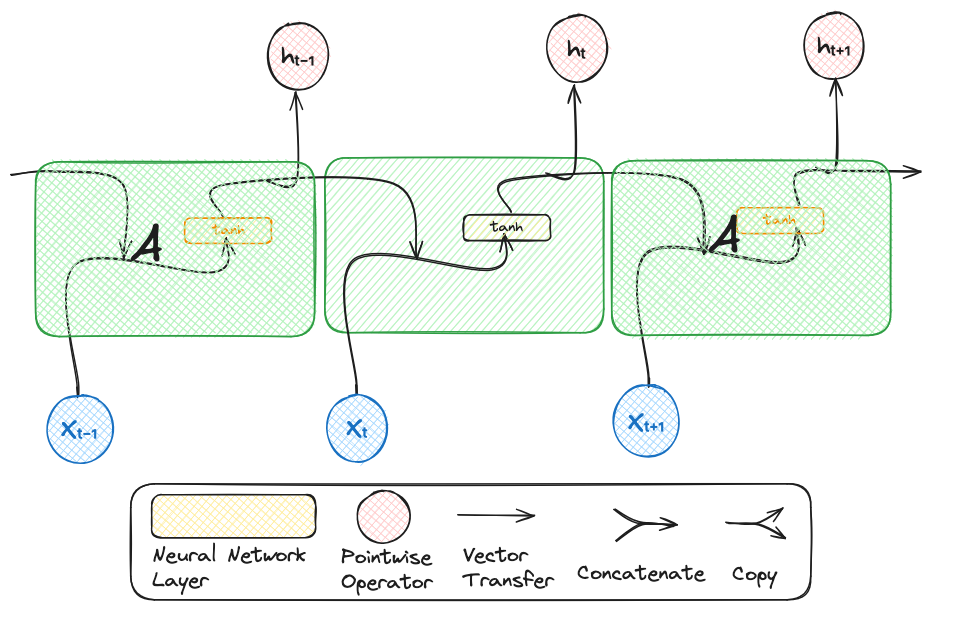
\includegraphics[width=9cm, height=6cm]{LSTM/images/LSTM1.png}
\end{center}

\begin{itemize}
    \item one green box is a single neural network layer which has a tanh activation function.
    \item The single neural network has two inputs:
    \begin{itemize}
        \item $X_t$ at time $t$ and 
        \item $h_{t-1}$  which is the output of the previous RNN block.
    \end{itemize} 
    \item $tanh$ is applied to the concatenation of the two inputs 
    \item The output is:
    \begin{itemize}
        \item $h_t$ as an ouput as well as 
        \item $h_t$ is the input to the next RNN block
    \end{itemize}
\end{itemize}
The above is the vanilla RNN. 
%************************************************************************************
\section{LSTM}
%************************************************************************************
Long Short-term Memory (LSTM) is capable of modeling longer term dependencies by having \textcolor{red}{memory cells} and \textcolor{red}{gates} that controls the information flow along with the memory cells.
Let us now draw a parallel with LSTM which has a similar structure.\\
\begin{center}
  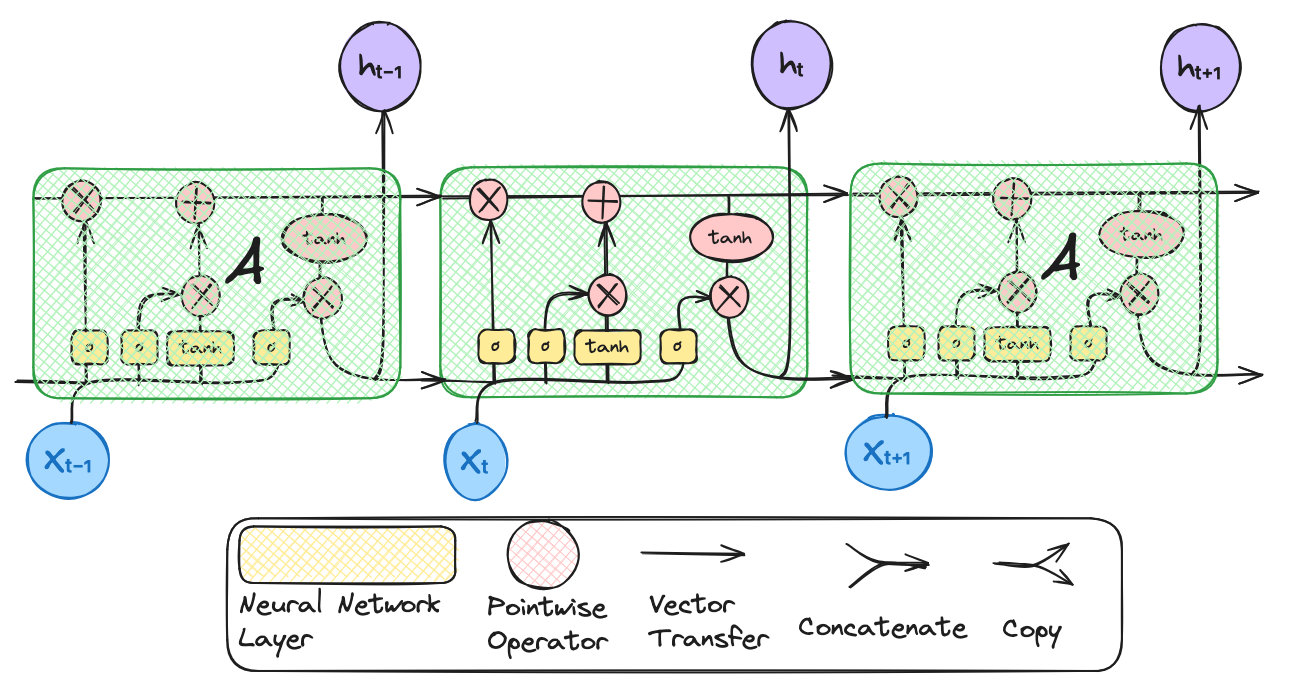
\includegraphics[width=9cm, height=6cm]{LSTM/images/LSTM2.png}   
\end{center}

\begin{itemize}
    \item All RNNs have the form of a chain of repeating modules of neural network
    \item Repeating module in an LSTM contains four interacting layers. They are not sequential layers unlike the network that we have seen so far. They also interact with each other. 
\end{itemize}
\begin{center}
    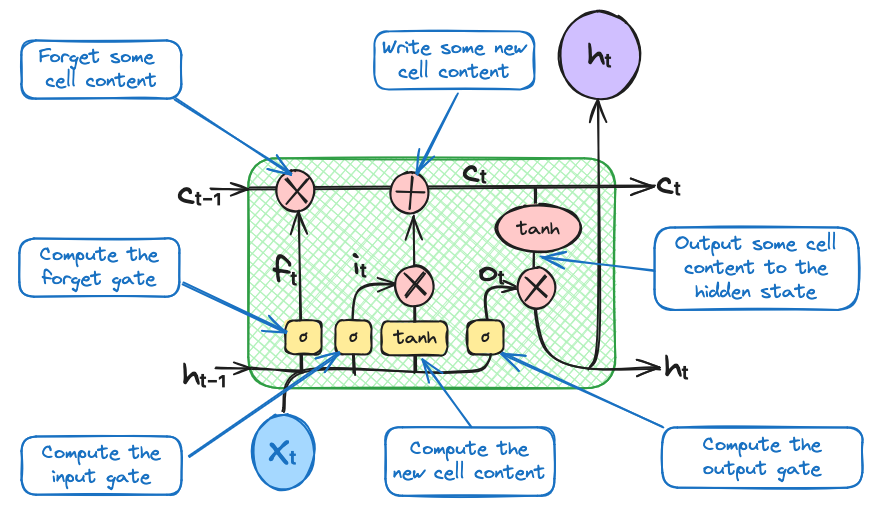
\includegraphics[width=9cm, height=6cm]{LSTM/images/LSTM3.png} 
\end{center}

The content of the \textcolor{red}{memory cells}, $C_t$, are regulated by 4 different gates which are also the four  different layers in a block (denoted by yellow boxes):
\begin{itemize}
    \item \textcolor{red}{\textit{Forget Gate}}, $f_t$, which decides to forget some cell content coming from the previous state. 
    \item \textcolor{red}{\textit{Input Gate}}, $i_t$, along with $tanh$ activation function decides how much of the input should be written and it also adds the cell content in the end
    \item \textcolor{red}{\textit{Output Gate}},$o_t$,  which decides how much of the cell state, $c_t$ should be exposed as the hidden state $h_t$. A part of $c_t$ is revealed as $h_t$ to the next time step as well an output of teh cell for further processing. 
    \item \textcolor{red}{\textit{Reset Gate}},$r_t$,
\end{itemize}
Each gates are composed of \textit{affine transformation} with Sigmoid activation function. The reason we use the Sigmoid activation function is that we want the output to lie between 0 and 1. 
\subsection{LSTMs explained}
\begin{center}
  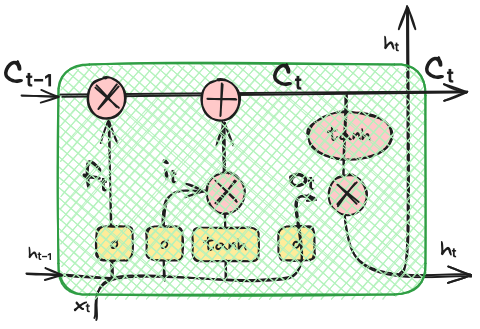
\includegraphics[width=9cm, height=6cm]{LSTM/images/CellState.png}  
\end{center}
%************************************************************************************
\subsubsection{Cell State $C_t$ \& Gates}
The cell state contains information which is a memory across a temporal context. The information can flow across the cell state unchanged. This is important from the perspective of vanishing gradient. The multiplication operator decides whether you want to forget something from a previous cell state $C_{t-1}$. The operator contains a sigmoid neural network layer which has a dimension as the size of the cell state and has a value between 0 and 1 for each dimension of that cell state. For each dimension of the cell state you can decide how much of the information you want to retain using the multiplication operator. This multiplication operation is a pointwise or elementwise multiplication operation. \\ 
\textcolor{red}{\textit{What does the multiplication operator in the cell state path do?}}\\
\textcolor{MidnightBlue}{The \textit{multiplication operator} decides decides whether you want to forget something from the previous cell state.} \\
\textcolor{red}{\textit{What does the addition operator in the cell state path do?}}\\
\textcolor{MidnightBlue}{The \textit{addition operator} decides how much of the new information gets added to the cell state.} \\
\textcolor{red}{\textit{What does the sigmoid neural net layer in the cell state do?}}\\
\textcolor{MidnightBlue}{The sigmoid neural net layer along with pointwise multiplication operation decides how much of each component from the previous cell state $C_{t-1}$ should be let through (remembered or forgotten?). } \\
%************************************************************************************
\subsubsection{Forget Gate}
\begin{itemize}
    \item Forget Gate is one of the layers inside the LSTM block. It determines how much contents from previous cell state $C_{t-1}$ will be \textcolor{red}{erased}.
    \item Linear transformation of concatenated previous hidden states and input are followed by Sigmoid activation function.
    $$ f_t = \sigma (W_f \cdot [h_{t-1}, x_t] + b_f) $$
    \item The sigmoid activation function generates values between 0 and 1:
    \begin{itemize}
        \item 0: completely remove info in the dimension
        \item 1: completely keep info in the dimension
    \end{itemize}
\end{itemize}
 

\textcolor{red}{\textit{What does the forget gate do?}}\\
\textcolor{MidnightBlue}{Forget gate $f_t$ does elemnt wise multiplication with the previous cell state $C_{t-1}$ to decide how much of that information should be erased and how much of teh information should be kept. } \\



%************************************************************************************
\subsubsection{Input Gate \& Cell Content}
\begin{itemize}
    \item \textcolor{red}{\textit{Cell Content/ New Candidate Cell}}, $\tilde{C}_t $: New content to be written to the cell. $\tilde{C}_t$ is created as a function of $h_{t-1}$ and $x_t$.\\
                    $$ \tilde{C}_t = tanh(W_C \cdot [h_{t-1}, x_t] + b_C)  $$
    \item \textcolor{red}{\textit{Input Gate}}, $i_t$,: decides how much of values of the new candidate cell sattes $\tilde{C}_t$ are combined into the cell states.\\
                    $$i_t = \sigma(W_i \cdot [h_{t-1}, x_t] + b_i)  $$
\end{itemize}


We have the $tanh$ activation function so that we get both negative and positive values. 
%************************************************************************************
\subsubsection{Update Cell State}
\textcolor{red}{\textit{Cell State}}: The previous cell states $C_{t-1}$ are updated to the new cell states $C_t$ by using the input and forget gates with new candidate cell states:  erase ("forget") some content from last cell state, and write ("input") some new cell content.
$$ C_t = f_t \ast C_{t-1} + i_t \ast \tilde{C}_t  $$
%************************************************************************************
\subsubsection{Output Gate and Hidden State}
\begin{itemize}
    \item Output is based on cell state $C_t$ with filter fromn the output gate $o_t$
    \item \textcolor{red}{\textit{Output Gate}}, $o_t$: decides which part of cell state $C_t$ are output to the hidden state, $h_t$
    $$o_t = \sigma(W_o [h_{t-1}, x_t] + b_o) $$
    \item \textcolor{red}{\textit{Hidden State}}, $h_t$: Then the \textcolor{red}{final output},  $h_t$, is generated from tanh-ed cell states filtered by $o_t$
    $$ h_t = o_t \ast tanh(C_t)$$
\end{itemize}



%*********************************************************************************************
\subsection{LSTM Summary}
\begin{itemize}
    \item \textcolor{blue}{\textit{Forget Gate}}: $f_t$ controls what is kept vs forgotten, from previous cell state
    \item \textcolor{blue}{\textit{Input Gate}}: $i_t$ controls what parts of the new cell content are written to cell
    \item \textcolor{blue}{\textit{Output Gate}}: $o_t$ controls what parts of the cell are output to the hidden state
    \item \textcolor{blue}{\textit{ Sigmoid function}}: all the above gate values are between 0 and 1
\end{itemize}

\begin{align*}
    f_t &= \sigma(W_f \cdot [h_{t-1},x_t] + b_f)\\
    i_t &= \sigma(W_i \cdot [h_{t-1}, x_t] + b_i) \\
    o_t &= \sigma(W_o \cdot [h_{t-1}, x_t] + b_o)
\end{align*} \\

\begin{itemize}
    \item \textcolor{blue}{\textit{ New Cell Content}}: this is the new cell content to be written to the cell
    \item \textcolor{blue}{\textit{ Cell State}}: erase ("forget") some content from the last cell state, and write ("input) some new cell content
    \item \textcolor{blue}{\textit{ Hidden State}}: read ("output") some content from the cell 
\end{itemize}
\begin{align*}
    \tilde{C}_t &= tanh(W_c \cdot [h_{t-1}, x_t] +b_c )\\
    C_t &= f_t \ast C_{t-1} + i_t \ast \tilde{C}_t \\
    h_t &= o_t \ast tanh(C_t)
\end{align*}

\textcolor{red}{\textit{Q. What can you tell about cell state $C_t$, if forget gate is set to 1 and input gate set to 0?}}\\
\textcolor{blue}{\textit{Information of that cell is \textbf{preseved indefinitely}}}\\
\textcolor{red}{\textit{Q. What happens if you fix input gate to all 1s, forget gate to all 0s, output gate to all 1s}}\\
\textcolor{blue}{\textit{Almost \textbf{standard RNN}}}\\
%************************************************************************************
\section{References}
%************************************************************************************
\begin{itemize}
    \item \href{https://www.youtube.com/watch?v=4vryB1QhBNc}{NPTEL Lecture}
    \item \href{https://people.cs.pitt.edu/~jlee/papers/cs3750_rnn_lstm_slides.pdf}{Pitt Notes}
\end{itemize}
\end{document}